% abtex2-modelo-artigo.tex, v-1.9.2 laurocesar
% Copyright 2012-2014 by abnTeX2 group at http://abntex2.googlecode.com/ 
%

% ------------------------------------------------------------------------
% ------------------------------------------------------------------------
% abnTeX2: Modelo de Artigo Acadêmico em conformidade com
% ABNT NBR 6022:2003: Informação e documentação - Artigo em publicação 
% periódica científica impressa - Apresentação
% ------------------------------------------------------------------------
% ------------------------------------------------------------------------




\documentclass[
	% -- opções da classe memoir --
	article,			% indica que é um artigo acadêmico
	11pt,				% tamanho da fonte
	oneside,			% para impressão apenas no verso. Oposto a twoside
	a4paper,			% tamanho do papel. 
	english,			% idioma adicional para hifenização
	brazil,				% o último idioma é o principal do documento
	sumario=tradicional
	]{abntex2}


% ---
% PACOTES
% ---

% ---
% Pacotes fundamentais 
% ---
\usepackage{lmodern}			% Usa a fonte Latin Modern
\usepackage[T1]{fontenc}		% Selecao de codigos de fonte.
\usepackage[utf8]{inputenc}		% Codificacao do documento (conversão automática dos acentos)
\usepackage{indentfirst}		% Indenta o primeiro parágrafo de cada seção.
\usepackage{nomencl} 			% Lista de simbolos
\usepackage{color}				% Controle das cores
\usepackage{graphicx}			% Inclusão de gráficos
\usepackage{microtype} 			% para melhorias de justificação
\usepackage{listings}

% ---
		
% ---
% Pacotes adicionais, usados apenas no âmbito do Modelo Canônico do abnteX2
% ---
\usepackage{lipsum}				% para geração de dummy text
% ---
		
% ---
% Pacotes de citações
% ---
\usepackage[brazilian,hyperpageref]{backref}	 % Paginas com as citações na bibl
\usepackage[alf]{abntex2cite}	% Citações padrão ABNT
% ---

% ---
% Configurações do pacote backref
% Usado sem a opção hyperpageref de backref
\renewcommand{\backrefpagesname}{Citado na(s) página(s):~}
% Texto padrão antes do número das páginas
\renewcommand{\backref}{}
% Define os textos da citação
\renewcommand*{\backrefalt}[4]{
	\ifcase #1 %
		Nenhuma citação no texto.%
	\or
		Citado na página #2.%
	\else
		Citado #1 vezes nas páginas #2.%
	\fi}%
% ---

% ---
% Informações de dados para CAPA e FOLHA DE ROSTO
% ---
\titulo{Planejamento de software - \textit{FixCodeApp}}
\autor{
Diego F. de Sousa$^{1}$, Bruno L. de Alcântara$^{1}$\\
\\
$^{1}$Curso Bacharelado em Sistemas de Informação -- Universidade Federal do Piauí\\
\texttt{\{diegofernando5672, brunolopes.ips\}@gmail.com}
\\\\\\\\\\\\\\\\\\\\
O objetivo geral deste trabalho é documentar todo \\
o processo de projeto da aplicação \textit{FixCodeApp} para a disciplina\\ de Projeto e Desenvolvimento de Sistemas de Informação I \\
sob a orientação do professor Filipe Fontinele \\
\\\\\\\\\\\\\\\\\\\\\\\\\\\\\\\\\\\
}
% ---

% ---
% Configurações de aparência do PDF final

% alterando o aspecto da cor azul
\definecolor{blue}{RGB}{41,5,195}

% informações do PDF
\makeatletter
\hypersetup{
     	%pagebackref=true,
		pdftitle={\@title}, 
		pdfauthor={\@author},
    	pdfsubject={Modelo de artigo científico com abnTeX2},
	    pdfcreator={LaTeX with abnTeX2},
		pdfkeywords={abnt}{latex}{abntex}{abntex2}{atigo científico}, 
		colorlinks=true,       		% false: boxed links; true: colored links
    	linkcolor=blue,          	% color of internal links
    	citecolor=blue,        		% color of links to bibliography
    	filecolor=magenta,      		% color of file links
		urlcolor=blue,
		bookmarksdepth=4
}
\makeatother
% --- 

% ---
% compila o indice
% ---
\makeindex
% ---

% ---
% Altera as margens padrões
% ---
\setlrmarginsandblock{3cm}{3cm}{*}
\setulmarginsandblock{3cm}{3cm}{*}
\checkandfixthelayout
% ---

% --- 
% Espaçamentos entre linhas e parágrafos 
% --- 

% O tamanho do parágrafo é dado por:
\setlength{\parindent}{1.3cm}

% Controle do espaçamento entre um parágrafo e outro:
\setlength{\parskip}{0.2cm}  % tente também \onelineskip

% Espaçamento simples
\SingleSpacing

% ----
% Início do documento
% ----
\begin{document}

% Retira espaço extra obsoleto entre as frases.
\frenchspacing 

% ----------------------------------------------------------
% ELEMENTOS PRÉ-TEXTUAIS
% ----------------------------------------------------------


% página de titulo
\maketitle
\tableofcontents
\newpage 


% ]  				% FIM DE ARTIGO EM DUAS COLUNAS
% ---

% ----------------------------------------------------------
% ELEMENTOS TEXTUAIS
% ----------------------------------------------------------
\textual

% ----------------------------------------------------------
% Introdução
% ----------------------------------------------------------
\section{Contexto}
Nesta seção será mostrado todo o embasamento para contextualizar o projeto. Esta parte sustenta as demais apresentando e explicando o que é a aplicação \textit{FixCodeApp}.

\subsection{Contextualização do Projeto}

Ao longo do tempo, a computação se tornou uma das áreas de estudos mais promissoras do mundo. Este fato se deve a crescente demanda tecnológica que circula entre as empresas e grupos de pesquisa. As subáreas que envolvem a programação e o desenvolvimento figuram entre as mais requisitadas do mercado fazendo com que mais e mais pessoas se interessem pela Tecnologia da Informação como um todo.

O mercado da TI no Brasil emprega 1,3 milhão de pessoas e de acordo com a Associação Brasileira de Empresas de Tecnologia da Informação e Comunicação, 50 mil pontos de trabalho estão esperando por um profissional qualificado\footnote{Mercado de TI é um dos setores que não pararam de contratar no Brasil. \cite{g1}}.

A matéria que foi publicada no G1 retrata a realidade da TI no Brasil em uma ótica positiva. Porém as vagas existem pois falta gente preparada para assumir cargos nesta categoria. Talvez a falta de fortalecimento prático e teórico das habilidades dos desenvolvedores precisem de um certo empurrão.

A área da TI sempre estará em constante mudança e os desenvolvedores sempre se deparam em situações nas quais precisam de algum tipo de auxílio ou até mesmo querem compartilhar algo que descobriu e quer que outras pessoas também desfrutem da descoberta.

Recentemente foi desenvolvida uma plataforma com o intuito de somar esforços pensando no problema acima citado, esta recebeu o nome de \textit{FixCode}. O \textit{FixCode} se comporta como um meio de auxílio aos desenvolvedores e programadores permitindo o usuário poder, tanto sanar dúvidas com relação à algoritmos, como também expor projetos e ideias com possibilidade de fazer o \textit{upload} de arquivo.

Atualmente, o \textit{FixCode}\footnote{Site oficial do  \textit{FixCode} (\href{https://fixcode.herokuapp.com/}{https://fixcode.herokuapp.com/})} é uma plataforma \textit{web} escrita em basicamente em \textit{Python}. A iniciativa nasceu em meados de agosto do ano de 2016 quando um dos desenvolvedores da plataforma comentou a respeito de uma ferramenta que unisse os desenvolvedores e programadores a fim de que pudessem compartilhar conhecimento.
 
A versão final deste projeto (\textit{Web}) foi apresentada no dia 25/02/2017 para a disciplina de Programação para Web II na Universidade Federal do Piauí - Campus Senhor Helvídio Nunes de Barros.

\subsection{Objetivos do Projeto}

Atualmente no Brasil, 69\% dos acessos à internet são originados dos smartphones. Esta estatística é o reflexo da crescente valorização dos aparelhos móveis na tecnologia\footnote{Smartphone se consolida como meio preferido de acesso à internet, diz pesquisa. \cite{smart}}. 

Sabendo disso, o presente projeto visa a criação de uma aplicação mobile para a plataforma \textit{FixCode}.

O \textit{FixCodeApp}, como será batizado, terá o maior numero de funcionalidades possíveis em consonância ao projeto atual que está na plataforma \textit{web} para que o usuário possa ter a melhor experiência possível, além de outros benefícios consequentes como praticidade, rapidez e facilidade.

\section{Métodos}

Dividimos esta seção em duas partes. A primeira irá detalhar o como irá funcionar a aplicação mostrando funcionalidades e recursos. Já na segunda abordaremos a razão do recurso que irá ser utilizado.

\subsection{Qual Método Será Empregado na Construção}

O projeto se baseará em uma aplicação híbrida, esta irá consumir uma plataforma \textit{RESTful}. Isso irá prover as mesmas funcionalidades da plataforma \textit{Web} para a aplicação móvel.

Existem uma série de funções já estabelecidas na atual plataforma, podemos citar:

\begin{itemize}
	\item \textbf{Área de registro}: Onde o usuário poderá se cadastrar.
	\item \textbf{Linha do tempo}: Na \textit{timeline} aparecerá um misto de \textit{posts} e \textit{fixes}, sendo eles das pessoas seguidas e das pessoas das comunidades que você participa (vide habilidades). Os \textit{posts} e \textit{fixes} irão ser diferenciados talvez por uma sutil coloração.
	\item \textbf{Login e Logout}: O usuário entrará com seu \textit{username} e senha.
	\item\textbf{Edição de Perfil}: O usuário poderá inserir informações com bio, \textit{link} de perfil do \textit{GitHub} e Foto de Perfil.
	\item \textbf{Exibição de Fix e Post}: Mostrará a postagem e os candidatos a resposta correta (Árvore de comentários de 1 nível).
	\item \textbf{Área de perfil}: Exibição do perfil do usuário com suas respectivas informações, \textit{posts}, \textit{fixes} ao qual se relacionou, seguidores e seguindo. (Por questão de ética os \textit{fixes} criados por um usuário não serão exibidos no seu perfil).
	\item \textbf{Seguidores}: Exibirá a lista de seguidores de um determinado usuário.
	\item \textbf{Seguindo}: Exibirá a lista de perfis que o usuário segue.
	\item \textbf{Pesquisa}: A partir de uma ação no campo de pesquisa, será exibida uma página contendo todo o conteúdo relacionado a palavra-chave pesquisada, e até outros usuários.
	\item \textbf{Área de contato e \textit{feedback}}: Onde o usuário, sendo ele cadastrado ou não, poderá contactar os desenvolvedores da aplicação.
	
\end{itemize}

Estes recursos também estarão estabelecidos na aplicação híbrida via transferência de dados HTTP com o formato de mensagens JSON. A plataforma \textit{FixCode} servirá um \textit{WebService} que irá operar como uma API.

Poderemos exemplificar um determinado recurso como:

\begin{lstlisting}
		http://fixcode.herokuapp.com/fix/34/
\end{lstlisting}

Para um resultado:

\begin{lstlisting}
		{
		  "id":"34",
		  "titulo":"Melhorando OO em java",
		  "autor":"diego",
		  "q_respostas":"3",
		}
\end{lstlisting}

A aplicação terá a característica híbrida, isso que dizer que serão feitas versões para a maioria dos sistemas \textit{mobile}, como \textit{Android, IOS e Windows Phone}.

\subsection{Motodologia ágil}

A metodologia ágil escolhida para o projeto foi o XP (\textit{Extreme Programming}). O objetivo principal do XP é levar ao extremo um conjunto de práticas que são ditas como boas na engenharia de software. As práticas do XP são fundamentais em valores. Veremos cada um dos valores do XP. Entre os valores temos:

\begin{itemize}
	\item \textbf{Comunicação}: A comunicação enfatiza que devemos sempre estar se comunicando seja entre desenvolvedores ou com clientes. XP é organizado em práticas que não podem ocorrer se não houver comunicação. Outra forma de comunicação no XP é a Programação em pares, onde os desenvolvedores programam num mesmo computador, nesse formato de programação ambos estão contantemente se comunicando e trocando ideias.
	
	\item \textbf{Simplicidade}: é tentar fazer o mais simples possível e caso seja necessário faremos algo mais complexo amanhã. Muitas vezes algo é feito de forma completa e posteriormente não é mais sequer usado ou necessário.
	Fazendo um paralelo entre a simplicidade e a comunicação conclui-se que a simplicidade faz com que temos menos a comunicar e de uma forma mais completa e por sua vez a comunicação faz com que transmitimos mais clareza e confiança para alimentar a simplicidade.
	
	\item \textbf{Feedback}: é muito presente no SCRUM através das reuniões diárias, retrospectivas, reuniões de revisão do produto, etc. O XP foi o percursor a falar em feedback e afirma que ele possibilita que o software evolua. O XP, como algo mais técnico que o SCRUM, diz que devemos sempre "Perguntar ao software, e não a um documento".
	
	\item \textbf{Coragem}: muitas vezes não fazemos as coisas porque não temos coragem de fazer as mudanças. XP diz que devemos ter coragem de sempre colocar o cliente a par do que está acontecendo.
	
	\item \textbf{Coach}: é uma pessoa responsável por garantir a aderência a estes valores nas práticas. O Coach normalmente é uma pessoa experiente que também ajuda as equipes a implementares o XP e monitorar se as coisas estão sendo bem seguidas.
\end{itemize}

\subsection{Qual o Motivo da Escolha}

Uma aplicação híbrida tem algumas vantagens sobre as aplicações nativas. Um exemplo claro disso é que o \textit{deploy} pode ser feita para várias plataformas, tanto \textit{mobile} como \textit{desktop}. No nosso caso, faremos para as plataformas mobile\textit{ Android, IOS e Windows Phone}. Outra vantagem das aplicações híbridas é que o desenvolvedor que tem conhecimentos sobre as tecnologias voltadas para \textit{web} (HTML, CSS e \textit{JavaScript}) tem caminho facilitado para o desenvolvimento, pois estas tecnologias são a principal base para a construção das aplicações.

Para metodologia ágil escolhemos os XP por conta da sua versatilidade e por ser voltada para equipes pequenas, assim ela poderá haver uma sintonia em conjunto a carga horária dos desenvolvedores da aplicação.

\section{Análise de Riscos}

\subsection{A Identificação dos Risco }

Os prováveis riscos que podem acontecer no decorrer do projeto, são definidos pela falta de orçamento e cumprimento de cronogramas, por problemas técnicos durante a implementação das funcionalidades do aplicativo ou até mesmo durante a criação da interface, problemas com os servidores de teste com limite de acesso com corrente que ocasiona o derrubamento do site. Outro grande risco que pode acontecer, é na construção do aplicativo que não atendas todas as necessidades dos usuários em questão, como também a usabilidade e design do site podem prejudicar os usuários durante a sua utilização. 

\subsection{Projeção dos Riscos}

O impacto que os ricos podem ocasionar durante o desenvolvimento do aplicativo iram prejudicar de alguma forma a conclusão do mesmo. Caso aconteça riscos técnicos no decorrer da implementação, poderá afetar diretamente a conclusão correta do cronograma. Outro impacto, é se o aplicativo não atendas todas as necessidades dos usuários, pois se o site não atender suas exigências a finalidade da rede social (\textit{FixCode}) perderá seu uso, Além disso, caso o site consiga mais usuários acessando, poderá sendo derrubado por conta do limite que servidores pagos propõe.

\subsection{Avaliação dos Riscos}

Se acontecer um desses problemas definidos acima, a prioridade será tentar reavaliar as funcionalidades utilizando um espaço dentro do site onde eles podem dar dicas e sugestões que realmente atenda às suas necessidades, fazendo uma avaliação das dicas e sugestões enviadas podemos melhores o site e o aplicativo, evitando assim possíveis transtornos. Se algum problema técnico acontecer, o ideal é tentar resolvê-lo imediatamente, em questão dos servidores, procurar melhor ou transferir o site para servidores melhores. Dessa forma o cumprimento correto do cronograma que seria no caso aplicativo.

\subsection{Administração e Monitoração dos Riscos}

Durante a administração e monitoração dos ricos serão realizadas técnicas para garantir a continuidade do projeto, fazendo um planejamento adequado dos requisitos a serem implementados, sempre atendendo as necessidades dos usuários para que eles sempre se sintam satisfeitos com o site e o aplicativo.

\section{Cronograma }

Nesta seção, serão descritos os esforços planejados para a construção da ferramenta proposta e sua duração prevista, de forma a promover uma maior organização na execução dos conjuntos de tarefas. 

\subsection{Relação Pessoa/Trabalho}

Aqui são descritas de forma sucinta as participações dos integrantes da equipe de desenvolvimento na construção da ferramenta proposta. 

\textbf{Diego Fernando} – Idealizador, Gerente de Projeto e Programador terá como função no âmbito de desenvolvimento de promover a integração entre a API e a plataforma principal (\textit{FixCode}) e conectá-la ao aplicativo móvel, além de assumir o papel administrativo do processo de desenvolvimento com a gerência do projeto e XP master.

\textbf{Bruno Lopes} – Programador e Auxiliar Administrativo, por sua vez terá responsabilidade sobre a documentação do projeto e quaisquer elementos burocráticos necessários à implementação da ferramenta, além do desenvolvimento da aplicação (cliente), funcionalidades e atualização de versões subsequentes da ferramenta.

\subsection{Definição de Tarefas}

Apesar de as responsabilidades gerais serem relatadas no tópico anterior, aqui podem ser notadas as especificações de cada tarefa relacionada ao desenvolvimento da aplicação.

Neste panorama levamos em consideração os vários aspectos relativos ao desenvolvimento, deixamos em voga a parte da codificação da aplicação \textit{mobile}. Esta ficará com a carga maior de 60 dias.

Outra parte bastante importante é a análise e/ou especificação. Começamos desde o início da disciplina a cogitar o rol de tecnologias que farão parte do projeto.

Integrar o aplicativo a API também promete ser custoso. Por isso os testes serão com a API desenvolvida localmente para evitar maiores problemas. Deixamos 12 dias para o estudo da API. Este tempo será destinado para uma reflexão de como será construída a arquitetura REST na plataforma.

\begin{table}[h]
	\centering
	\caption{Tarefas}
	\label{my-label}
	\begin{tabular}{|c|c|c|}
		\hline
		\textbf{Tarefa}               & \textbf{Estimativa de Duração} & \textbf{Índice de Criticidade} \\ \hline
		Análise/Especificação         & 30 dias                        & A                              \\ \hline
		Revisão de Requisitos         & 15 dias                        & B                              \\ \hline
		Revisão do Projeto Preliminar & 10 dias                        & B                              \\ \hline
		Codificação                   & 60 dias                        & A                              \\ \hline
		Testes Unitários              & 5 dias                         & D                              \\ \hline
		Estudo para Integração da API & 12 dias                        & A                              \\ \hline
		Desenvolvimento da API        & 5 dias                         & A                              \\ \hline
		Testes de Integração          & 3 dias                         & D                              \\ \hline
		Implementação da API          & 3 dias                         & A                              \\ \hline
		Testes de Integração          & 4 dias                         & D                              \\ \hline
		Validação                     & 3 dias                         & D                              \\ \hline
	\end{tabular}
\end{table}

\newpage

\subsection{Rede de Tarefas}

Para facilitar a compreensão da execução deste projeto, abaixo se apresenta uma rede de tarefas que ilustra o andamento planejado.

\begin{figure}[h]
	\label{figura1} 
	\caption{Rede de Tarefas}
	\centering 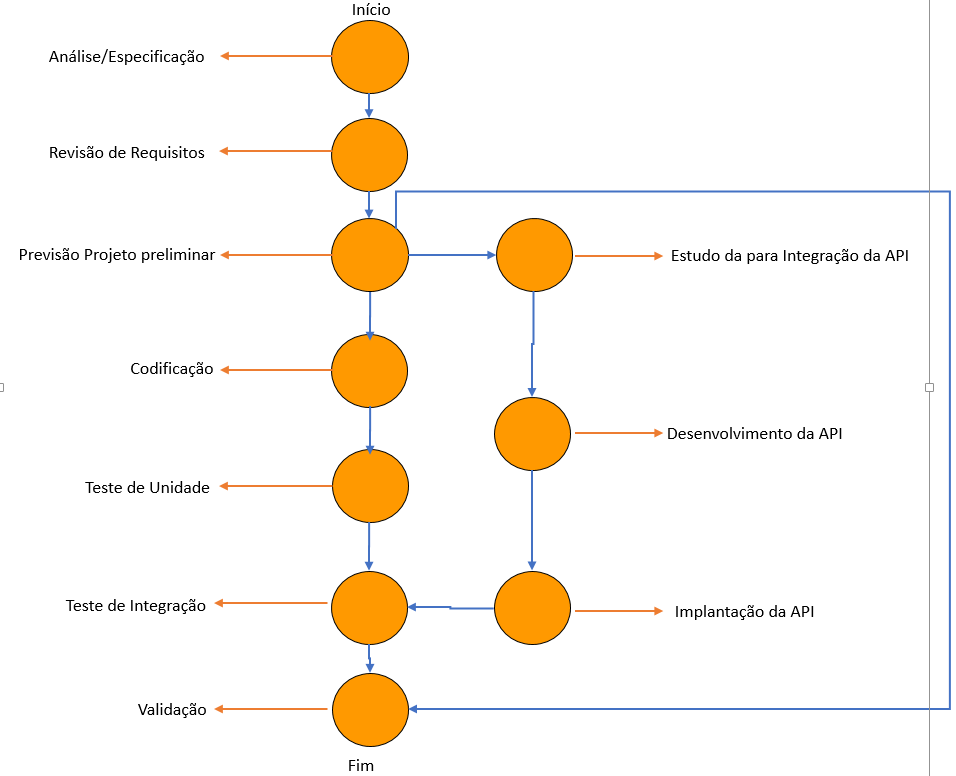
\includegraphics[width=0.90\textwidth]{rede.png}
\end{figure}

\subsection{Distribuição de Esforços}

De acordo com os períodos de tempo previstos para cada conjunto de atividades, abaixo nota-se a divisão de esforço estimada para a realização do projeto.

\begin{table}[h]
	\centering
	\caption{Esforços}
	\label{my-label}
	\begin{tabular}{|c|c|c|c|c|}
		\hline
		\textbf{Planejamento} & \textbf{\begin{tabular}[c]{@{}c@{}}Especificaçao \\ e Análise de\\ Requisitos\end{tabular}} & \textbf{Projeto} & \textbf{Implementação} & \textbf{Teste e Publicação} \\ \hline
		Até 5\%               & De 10\% a 25\%                                                                              & De 20\% a 25\%   & De 30\% a 40\%         & De 15\% a 20\%              \\ \hline
	\end{tabular}
\end{table}

\subsection{Representação do Cronograma}

A divisão temporal para execução do projeto se dará conforme representado na tabela a seguir.

\begin{table}
	\centering
	\caption{Cronograma}
	\label{my-label}
	\begin{tabular}{|c|c|c|c|c|c|}
		\hline
		& \textbf{Mês 1} & \textbf{Mês 2} & \textbf{Mês 3} & \textbf{Mês 4} & \textbf{Mês 5} \\ \hline
		Análise/Especificação & X              &                &                &                &                \\ \hline
		Planejamento          &                & X              &                &                &                \\ \hline
		Codificação           &                &                & X              & X              &                \\ \hline
		Testes                &                &                &                &                & X              \\ \hline
		Validação             &                &                &                &                & X              \\ \hline
	\end{tabular}
\end{table}

A tabela acima possui períodos mensais divididos em semanas para definir claramente os períodos planejados para cada etapa do desenvolvimento.

\section{Planejamento Organizacional}

A equipe de desenvolvimento se baseará na metodologia ágil XP, mas estará sempre aberta a novas sugestões tanto por parte dos atuais usuários da plataforma \textit{Web}, como também qualquer pessoa que queira ter sua opinião registrada.

Ao momento que o processo de desenvolvimento for chegando em sua reta final faremos a aplicação beta passará por fazes de testes com usuários reais. E assim permanecerá para coleta de dados a fim de melhorar a aplicação.

A equipe também estará sempre antenada sobre as atualizações das tecnologias que irão ser usadas no desenvolvimento como também estará sempre atenta nas novas tecnologias que surgem para garantir eficiência na performance da aplicação.

Manter a documentação da API sempre atualizada também está no planejamento, assim como manter o aplicativo com uma Experiência de Usuário melhor.

\section{Recursos Necessários}

Para este tópico, têm-se a separação dos principais recursos, humanos ou não, indispensáveis para a execução do projeto.

\subsection{Pessoal}

Estima-se a necessidade de apenas duas pessoas para o desenvolvimento da lógica e integrações do sistema, com a possível contratação de um consultor de Interfaces Gráficas para auxílio no desenvolvimento de uma interface suficientemente amigável. Além disso, almeja-se convidar pessoas para utilizar e dar suas opiniões, sugestões e dicas verificando a aceitação do aplicativo. 

\subsection{Software e Hardware}

A construção da ferramenta proposta demanda inicialmente a utilização de:

\begin{itemize}
	\item Pelo menos 3 smartphones, com os repectivos sistema operacional como Android e IOS e Windows Phone, para testar a aplicação;
	
	\item Um computador para o desenvolvimento do Aplicativo.
\end{itemize}

Para recursos lógicos:

\begin{itemize}
	\item \textbf{Django Rest Framework\footnote{Site oficial do  \textit{Django Rest Framework} (\href{http://www.django-rest-framework.org/}{http://www.django-rest-framework.org/})}}: \textit{Django Rest Framework} é uma extensão da famosa \textit{framework} para \textit{WEB Django}. A DRF (Abr.) auxilia na serialização dos componentes afim de se criar API’s \textit{Restful}. Terá grande importância pra o projeto, uma vez que o aplicativo \textit{mobile} irá consumir a API contruída nesta tecnologia.
	
	\item \textbf{PhoneGap/Cordova\footnote{Site oficial do \textit{Phonegap} (\href{https://phonegap.com/}{https://phonegap.com/})}}: Esta tecnologia é usada para criação de aplicações mobile híbridas. Ela será responsável por transformar todo o código que está nas tecnologias voltadas para \textit{WEB} (\textit{HTML, CSS, JavaScript}) para aplicações \textit{mobile}. 
	
	\item \textbf{Ionic}: O \textit{Ionic\footnote{Site oficial do \textit{Ionic} (\href{https://ionicframework.com/}{https://ionicframework.com/})}} é um \textit{framework} voltado para aplicações híbridas, que junto ao \textit{PhoneGap}, auxiliar á na navegabilidade dos componentes do aplicativos consumindo de forma eficiente os dados gerados da API \textit{Restful}
	
	\item \textbf{Tecnologias voltadas para a WEB}: Para a construção da aplicação \textit{mobile}, irão ser usadas as tecnologias voltadas para \textit{WEB: HTML, CSS, JavaScript}. Será eleita também uma \textit{framework frontend} para melhor praticidade no desenvolvimento da interface gráfica. Por enquanto, a mais cotada está sendo a \textit{MaterilizeCss}.
\end{itemize}

\section{Mecanismos de Acompanhamento}

Observando o fato de a equipe de desenvolvimento ser pequena, adota-se como principal mecanismo de acompanhamento para este projeto a execução de reuniões diárias para comparação do que foi produzido com o planejamento e quaisquer incrementos que possam ser sugeridos e verificados durante o processo de desenvolvimento. Obviamente, essa metodologia é cabível dada a metodologia ágil adotada para este projeto (XP) que possui um funcionamento baseado em incrementos constantes e posterior documentação.

% ----------------------------------------------------------
% Referências bibliográficas
% ----------------------------------------------------------
\newpage
\bibliography{abntex2-modelo-references}

\end{document}
